\documentclass [a4paper] {report}
\usepackage [utf8] {inputenc}
\usepackage [T1] {fontenc}
\usepackage [french] {babel}

%============================================================

\usepackage {minted}
\usepackage {graphicx}

%============================================================

\usepackage [style=numeric, sorting=ynt, natbib=true] {biblatex}
\addbibresource {rapport.bib}

%============================================================

\usepackage {array}
\usepackage {xspace}

%============================================================

\usepackage {amsmath}	% align*
\usepackage {amssymb}	% mathbb
\usepackage {mathrsfs}	% mathscr

%============================================================

\usepackage {mathpartir}
\def \RightTirNameStyle {\textnormal}

%============================================================

\usepackage {amsthm}

\newtheoremstyle {definition}
	{}		% space above
	{}		% space below
	{}		% body font
	{}		% indent
	{\bf}	% head font
	{\\}	% head punctuation
	{ }		% head space
	{}		% head spec

\newenvironment {preuve} 
	{\begin {proof} ~\\} 
	{\end {proof}}

\theoremstyle {definition}

\newtheorem {definition} {Définition} [section]
\newtheorem {lemme} {Lemme} [section]
\newtheorem {theoreme} {Théorème} [section]

%============================================================

\newcommand {\trie} {\textit {trie}}
\newcommand {\dowsindex} {\textit{dowsindex}\xspace}

\newcommand {\ssi} {\textit {ssi}\xspace}

\newcommand {\interval} [2] {[\![#1\,;#2]\!]}

\newcommand {\V} {\mathscr V}
\newcommand {\C} {\mathscr C}
\newcommand {\T} {\mathscr T}
\newcommand {\E} {\mathscr E}

\newcommand {\qeq} {\stackrel ? =}
\newcommand {\Eeq} {\stackrel \E =}
\newcommand {\ueq} {\stackrel u =}

%============================================================

\title {Recherche de fonctions \\ par \\ unification modulo isomorphismes de types}
\author {Clément ALLAIN}
\date {Juin 2021}

%============================================================

\begin {document}

\maketitle

\tableofcontents

\newpage

%============================================================
%============================================================

\chapter {Introduction}

S'il est une chose dont on a besoin en programmation fonctionnelle, c'est bien de fonctions. Seulement voilà, ce n'est pas si simple. Mettre la main sur l'une d'entre elles en présence d'un environnement de grande taille s'avère parfois difficile, à tout le moins fastidieux. Aussi, remédions.

Il s'agit de mettre sur pied un système de recherche de fonctions pour le langage OCaml. L'écosystème en est principalement composé des paquets OPAM --- des centaines de milliers d'identificateurs. Un tel outil épargnerait à l'utilisateur la peine de fouiller telle ou telle bibliothèque dans l'espoir d'y trouver une fonction s'accordant à son usage.

Mais que chercher et comment ? Des travaux similaires ont été menés notamment par Rittri pour Lazy ML \cite {rittri91, rittri93} et Delahaye pour Coq \cite {delahaye}. Nous empruntons à notre tour à Rittri \cite {rittri91} le tableau \ref {tab_fold}.

\begin {table} [h]
	\centering
	\begin {tabular} {|l|l|l|}
		\hline
			Langage &
			Nom &
			Type
		\\
		\hline
			LCF ML &
			\texttt {itlist} &
			$(\alpha \rightarrow \beta \rightarrow \beta) \rightarrow list (\alpha) \rightarrow \beta \rightarrow \beta$
		\\
			Caml &
			\texttt {list\_it} &
			$(\alpha \rightarrow \beta \rightarrow \beta) \rightarrow list (\alpha) \rightarrow \beta \rightarrow \beta$
		\\
			Haskell &
			\texttt {foldr} &
			$(\alpha \rightarrow \beta \rightarrow \alpha) \rightarrow \alpha \rightarrow list (\beta) \rightarrow \alpha$
		\\
			SML of New Jersey &
			\texttt {fold} &
			$(\alpha \times \beta \rightarrow \beta) \rightarrow list (\alpha) \rightarrow \beta \rightarrow \beta$
		\\
			Edinburgh SML &
			\texttt {fold\_right} &
			$(\alpha \times \beta \rightarrow \beta) \rightarrow \beta \rightarrow list (\alpha) \rightarrow \beta$ \\
		\hline
	\end {tabular}
	\caption {\label {tab_fold} Variations sur \texttt {list\_it} de Caml dans plusieurs langages fonctionnels}
\end {table}

Plusieurs observations en émanent. Une recherche par identificateur en l'espèce — une fonction se comportant comme \texttt {List.fold\_left} en OCaml — se heurterait à la diversité des noms potentiels. De même, une recherche syntaxique sur les types s'accommoderait mal des variations en un sens équivalentes de la forme du type. Pourtant, toutes ces fonctions font essentiellement le même travail ; cette diversité est due à l'arbitraire de l'auteur de la fonction.

Que faire, alors ? Une recherche par spécification s'avérerait bien plus satisfaisante, mais pas forcément décidable. On peut retenir comme spécification grossière le type d'une fonction — « \textit {type as search key} » — tout en l'enrichissant par une approche sémantique et non plus purement syntaxique. La \textit {recherche modulo isomorphisme de type} s'est imposée dans la littérature. Elle consiste intuitivement à autoriser des réarrangements triviaux dans les types : commutativité et associativité du produit, curryfication. Cette notion reste néanmoins à définir formellement, et surtout à décider algorithmiquement. Nous y consacrerons le chapitre 2.

Comme souligné par Rittri \cite {rittri93}, il est bienvenu d'autoriser l'instantiation des types dans la recherche. Si la chose est seulement permise aux types issus de l'écosystème, il s'agit de \emph {matching} ; si le type demandé peut aussi être instancié, on parlera d'\emph {unification}. Nous avons implémenté un algorithme d'unification préexistant \cite {boudet} présenté dans le chapitre 3.

Le système résultant ne saurait passer à l'échelle sans un travail sur les fonctions de l'écosystème préalable à la recherche. Nous discuterons de ces limites dans le chapitre 4. Nous y proposerons une technique d'indexation reposant sur des conditions nécessaires d'unifiabilité. L'apport de cette technique se révélera substantiel.

Enfin, nous décrirons dans le chapitre 5 le fruit de notre travail : l'outil  \dowsindex.

%============================================================
%============================================================

\chapter {Unification modulo isomorphismes de types}

\section {Isomorphismes de types}

La conception d'un outil de recherche de fonctions par types passe la construction d'une notion d'équivalence entre types. Les travaux de Mikael Rittri \cite {rittri91, rittri93} sur lesquels nous nous appuyons ont assis celle d'\emph{équivalence modulo isomorphismes de types}. La chose a fait l'objet de plusieurs recherches importantes, menées notamment par Giusseppe Longo, Kim Bruce, Roberto Di Cosmo \cite {bruce_dicosmo_longo, dicosmo92, dicosmo93, dicosmo95}, Sergei Soloviev \cite {soloviev83, soloviev93}, Paliath Narendran, Frank Pfenning et Richard Statman \cite {narendran_pfenning_statman}.

Plus précisément, ces travaux font référence aux isomorphismes de types dans plusieurs versions du $\lambda$-calcul simplement typé. En notant $=_{\beta \eta \pi *}$ l'égalité dans le $\lambda$-calcul simplement typé avec paires et élément terminal (voir par exemple \cite {dicosmo95} pour plus de détails), noté $\lambda^1 \beta \eta \pi *$, la notion d'isomorphisme de types dans ce calcul se définit ainsi :

\begin {definition} [isomorphisme de types dans $\lambda^1 \beta \eta \pi *$]
	Deux types $A$ et $B$ sont isomorphes dans $\lambda^1 \beta \eta \pi *$ \ssi il existe deux $\lambda$-termes $f : A \rightarrow B$ et $g : B \rightarrow A$ tels que $f \circ g =_{\beta \eta \pi *} \mathrm {id} _B$ et $g \circ f =_{\beta \eta \pi *} \mathrm {id} _A$.
\end {definition}

On peut donner une caractérisation équationnelle des isomorphismes de $\lambda^1 \beta \eta \pi *$ (voir la définition de théorie équationnelle dans l'annexe TODO). Ils correspondent aux isomorphismes valides dans les \emph {catégories cartésiennes fermées}. Giusseppe Longo, Kim Bruce, Roberto Di Cosmo \cite {bruce_dicosmo_longo} et Soloviev \cite {soloviev83} ont démontré par deux méthodes différentes que les axiomes équationnels ci-dessous sont corrects et complets ; on notera $Th^1 _{\times \bold T}$ la théorie équationnelle induite.
\begin {align*}
		A \times B &\cong
		B \times A &&
		\text {($\times$-comm)}
	\\
		A \times (B \times C) &\cong
		(A \times B) \times C &&
		\text {($\times$-assoc)}
	\\
		\bold T \times A &\cong
		A &&
		\text {($\times$-neutre)}
	\\
		(A \times B) \rightarrow C &\cong
		A \rightarrow (B \rightarrow C) &&
		\text {(curry)}
	\\
		\bold T \rightarrow A &\cong
		A &&
		\text {(curry-$\bold T$)}
	\\
		A \rightarrow (B \times C) &\cong
		(A \rightarrow B) \times (A \rightarrow C) &&
		\text {(dist)}
	\\
		A \rightarrow \bold T &\cong
		\bold T &&
		\text {(dist-$\bold T$)}
\end {align*}

Néanmoins, Paliath Narendran, Frank Pfenning et Richard Statman \cite {narendran_pfenning_statman} ont établi que, si le \emph {matching} modulo $Th^1 _{\times \bold T}$ est NP-complet, l'unification modulo $Th^1 _{\times \bold T}$ est indécidable. C'est ce qui a poussé Rittri \cite {rittri93} à se concentrer sur les cinq premiers axiomes correspondant aux isomorphismes \emph {linéaires} (voir \cite {rittri93} pour plus de détails) complets dans les \emph {catégories monoïdales fermées symétriques} \cite {soloviev93}. L'unification modulo cette nouvelle théorie est NP-complète \cite{narendran_pfenning_statman}. Cet abandon des deux axiomes de distributivité (dist) et (dist-$\bold T$) — et donc de la complétude dans $\lambda^1 \beta \eta \pi *$ — s'avère d'après lui bénin, arguant que ces isomorphismes sont peu utiles en pratique.

En outre, Di Cosmo \cite {dicosmo92} a étudié les isomorphismes de Core-ML. De même, il en a tiré une axiomatisation équationnelle complète comportant de nouveaux isomorphismes. L'équivalence est alors décidable par un algorithme qu'il introduit dans \cite {dicosmo95}. Bien que plus proche du langage OCaml qui nous intéresse, cet algorithme ne s'adapte a priori pas directement au matching ou l'unification.

Nous avons donc suivi les préconisations de Rittri en renonçant pour le moment à l'axiome (curry-$\bold T$). En effet, bien qu'utile en pratique pour simuler une expression paresseuse, nous avons préféré ne pas complexifier l'algorithme d'unification. Ne s'agissant pas de l'isomorphisme le plus important, cela affecte peu la qualité de la recherche. Les quatre isomorphismes restants sont donnés ci-dessous avec des types OCaml. Il est à noter que ces isomorphismes sont corrects pour Core-ML \cite {dicosmo93} et nous rendent optimistes quant à OCaml sans que cela soit démontré.
\begin {align*}
		\alpha * \beta &\cong
		\beta * \alpha &&
		\text {($*$-comm)}
	\\
		\alpha * (\beta * \gamma) &\cong
		(\alpha * \beta) * \gamma &&
		\text {($*$-assoc)}
	\\
		unit * \alpha &\cong
		\alpha &&
		\text {($*$-unit)}
	\\
		\alpha * \beta \rightarrow \gamma &\cong
		\alpha \rightarrow \beta \rightarrow \gamma &&
		\text {(curry)}
\end {align*}

TODO: exemples

\section {Unification sémantique}

L'égalité modulo isomorphisme étant décidable, on pourrait s'arrêter là et construire un outil de recherche testant l'équivalence des types. Une fois de plus inspirés par Rittri \cite {rittri93}, nous voulons autoriser non seulement les réarrangements mais aussi l'instanciation des types. Le matching — où seuls sont instanciés les types de l'environnement — comme l'unification — où le type demandé peut aussi être instancié — sont décidables \cite {narendran_pfenning_statman}. Nous avons choisi l'alternative la plus flexible : l'unification ; cependant, le matching s'y réduit. L'usage indique d'ailleurs qu'il n'est généralement pas souhaitable d'instancier le type demandé. C'est pourquoi nous en avons fait le comportement par défaut, avec la possibilité d'expliciter les variables de types instanciables.

TODO
\begin {itemize}
	\item état de l'art rapide unification sémantique AC
	\item présenter \cite {boudet}
	\item exemples avec dowsindex unify
\end {itemize}

%============================================================
%============================================================

\chapter {Indexation}

\section {Métriques de types}

\subsection {Nombre de variables}

TODO: retranscrire
\begin {figure} [h]
\begin {center}
	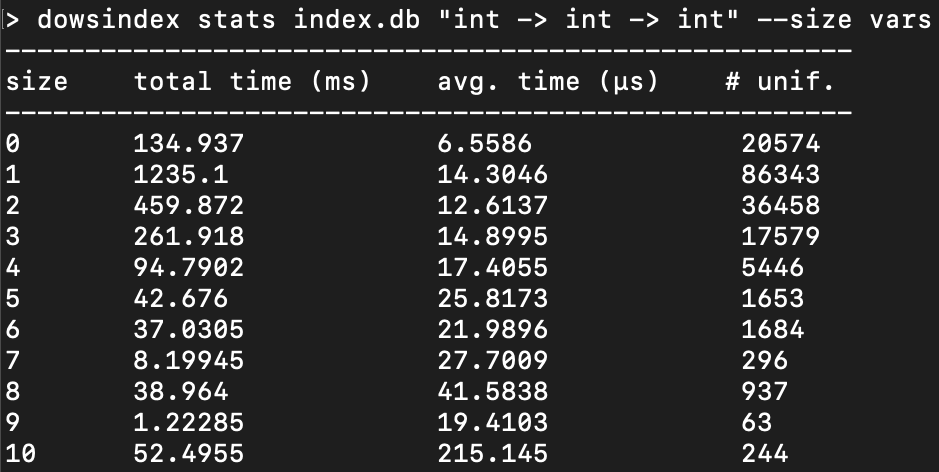
\includegraphics [scale=0.2] {images/stats1}
\end {center}
\end {figure}

TODO

\subsection {Type en tête}

TODO: retranscrire
\begin {figure} [h]
\begin {center}
	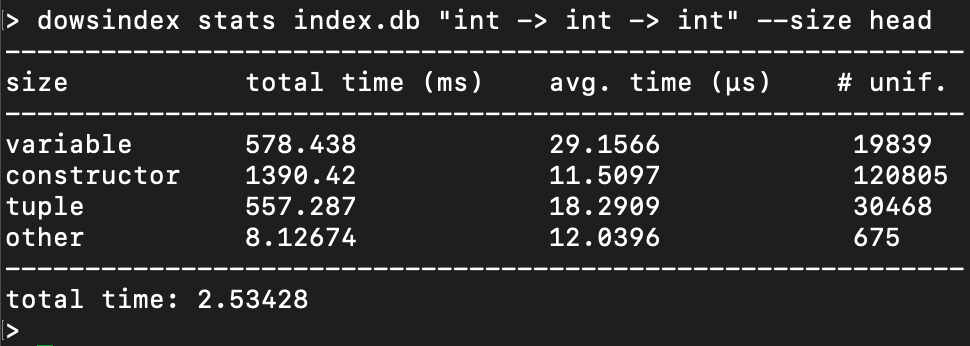
\includegraphics [scale=0.2] {images/stats2}
\end {center}
\end {figure}

TODO

\subsection {Nombre de variables dans la « colonne vertébrale »}

TODO: retranscrire
\begin {figure} [h]
\begin {center}
	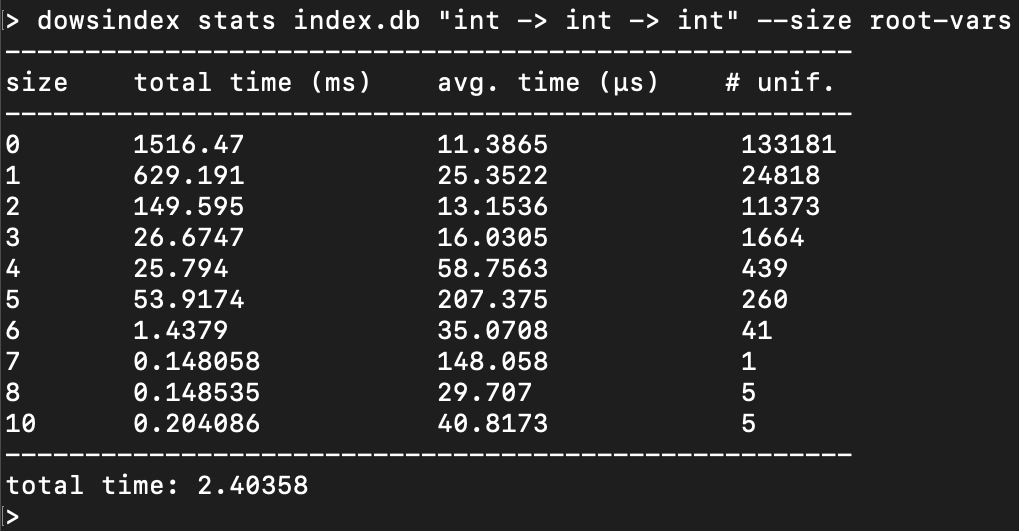
\includegraphics [scale=0.2] {images/stats3}
\end {center}
\end {figure}

TODO

\section {Conditions nécessaires d'unifiabilité}

\subsection {Premier critère (tête)}

\begin {figure} [h]
\begin {center}
	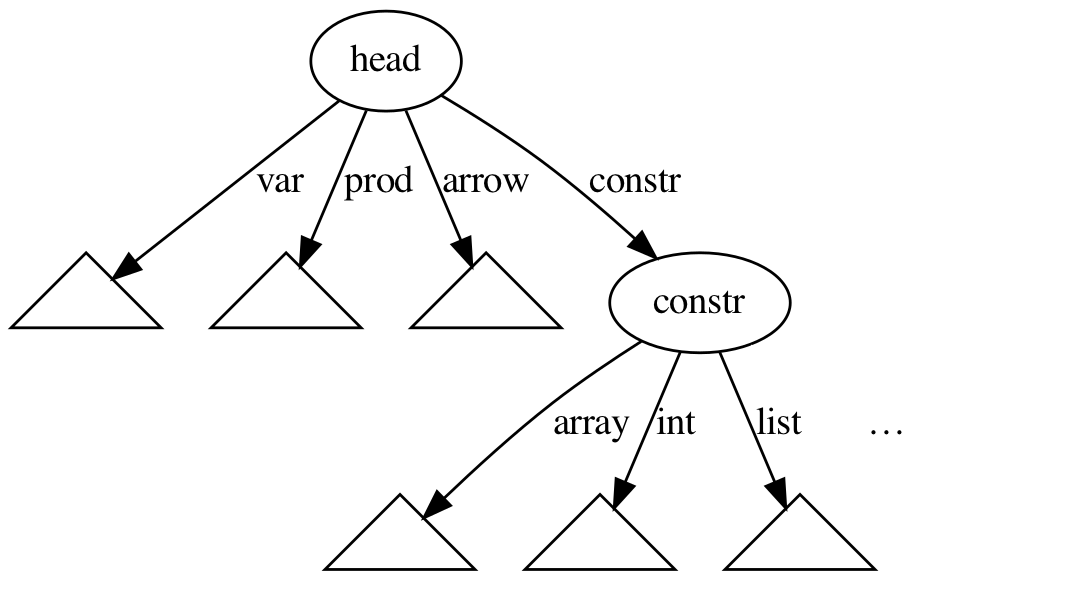
\includegraphics [scale=0.2] {graphs/by_head}
\end {center}
\end {figure}

TODO

\subsection {Deuxième critère (queue)}

TODO: graphe

TODO

\section {Structure de \trie}

\begin {figure} [h]
\begin {center}
	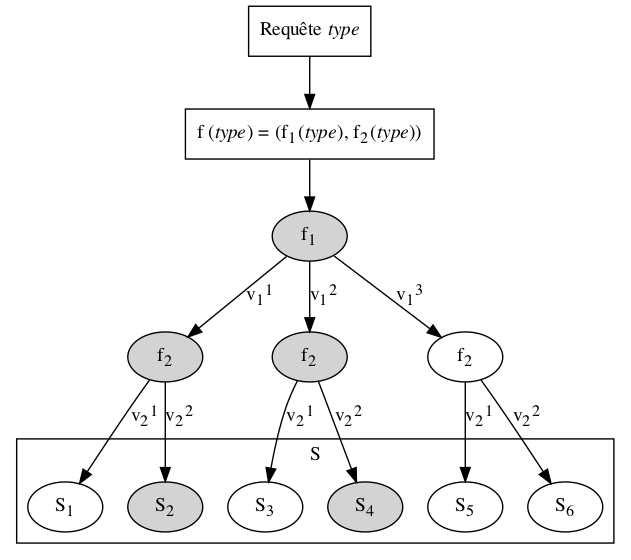
\includegraphics [scale=0.3] {graphs/trie}
\end {center}
\end {figure}

TODO
\begin {itemize}
	\item motivation avec \cite {schulz}
	\item exemples
\end {itemize}

%============================================================
%============================================================

\chapter {\dowsindex}

\begin {figure} [h]
\begin {center}
	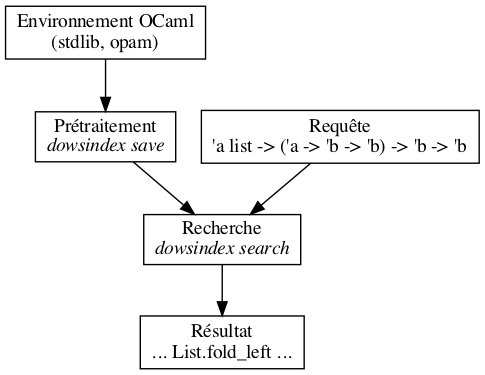
\includegraphics [scale=0.35] {graphs/dowsindex}
\end {center}
\end {figure}

\section {\dowsindex \textit {save}}

La commande \dowsindex \textit {save} admet les options suivantes :

\begin {table} [h]
\begin {tabular} {ll}
		\textbf{-{}-index}=\textit{fichier} &
		Sauvegarde l'index dans \textit {fichier}. \\ &
		Par défaut : dans un répertoire standard propre à stocker les données d'applications.
	\\
		\textbf {-{}-verbose} &
		Active le mode verbeux. Affiche les paquets trouvés.
\end {tabular}
\end {table}

TODO
\begin {itemize}
	\item présentation
	\item exemples : varier nombre de paquets, mise à jour
\end {itemize}

\section {\dowsindex \textit {stats}}

\begin {table} [h]
\begin {tabular} {ll}
		\textbf {-{}-filter} &
		Calcule aussi les statistiques avec filtrage par critères.
	\\
		\textbf{-{}-index}=\textit{fichier} &
		Cherche l'index dans \textit {fichier}. \\ &
		Par défaut : dans un répertoire standard propre à stocker les données d'applications.
	\\
		\textbf{-{}-measure}=\textit{mesure} &
		Mesure les types avec \textit {mesure}.
\end {tabular}
\end {table}

TODO
\begin {itemize}
	\item présentation
	\item exemples
\end {itemize}

\section {\dowsindex \textit {search}}

\begin {table} [h]
\begin {tabular} {ll}
		\textbf {-{}-exhaustive} &
		Recherche exhaustive (sans filtrage par critères).
	\\
		\textbf{-{}-index}=\textit{fichier} &
		Cherche l'index dans \textit {fichier}. \\ &
		Par défaut : dans un répertoire standard propre à stocker les données d'applications.
	\\
		\textbf {-n} \textit {n} &
		Affiche les \textit {n} premiers résultats seulement.
\end {tabular}
\end {table}

TODO
\begin {itemize}
	\item présentation
	\item exemples : varier nombre de paquets, types plus ou moins complexes
\end {itemize}

\section {Extensions}

\begin {figure} [h]
\begin {center}
	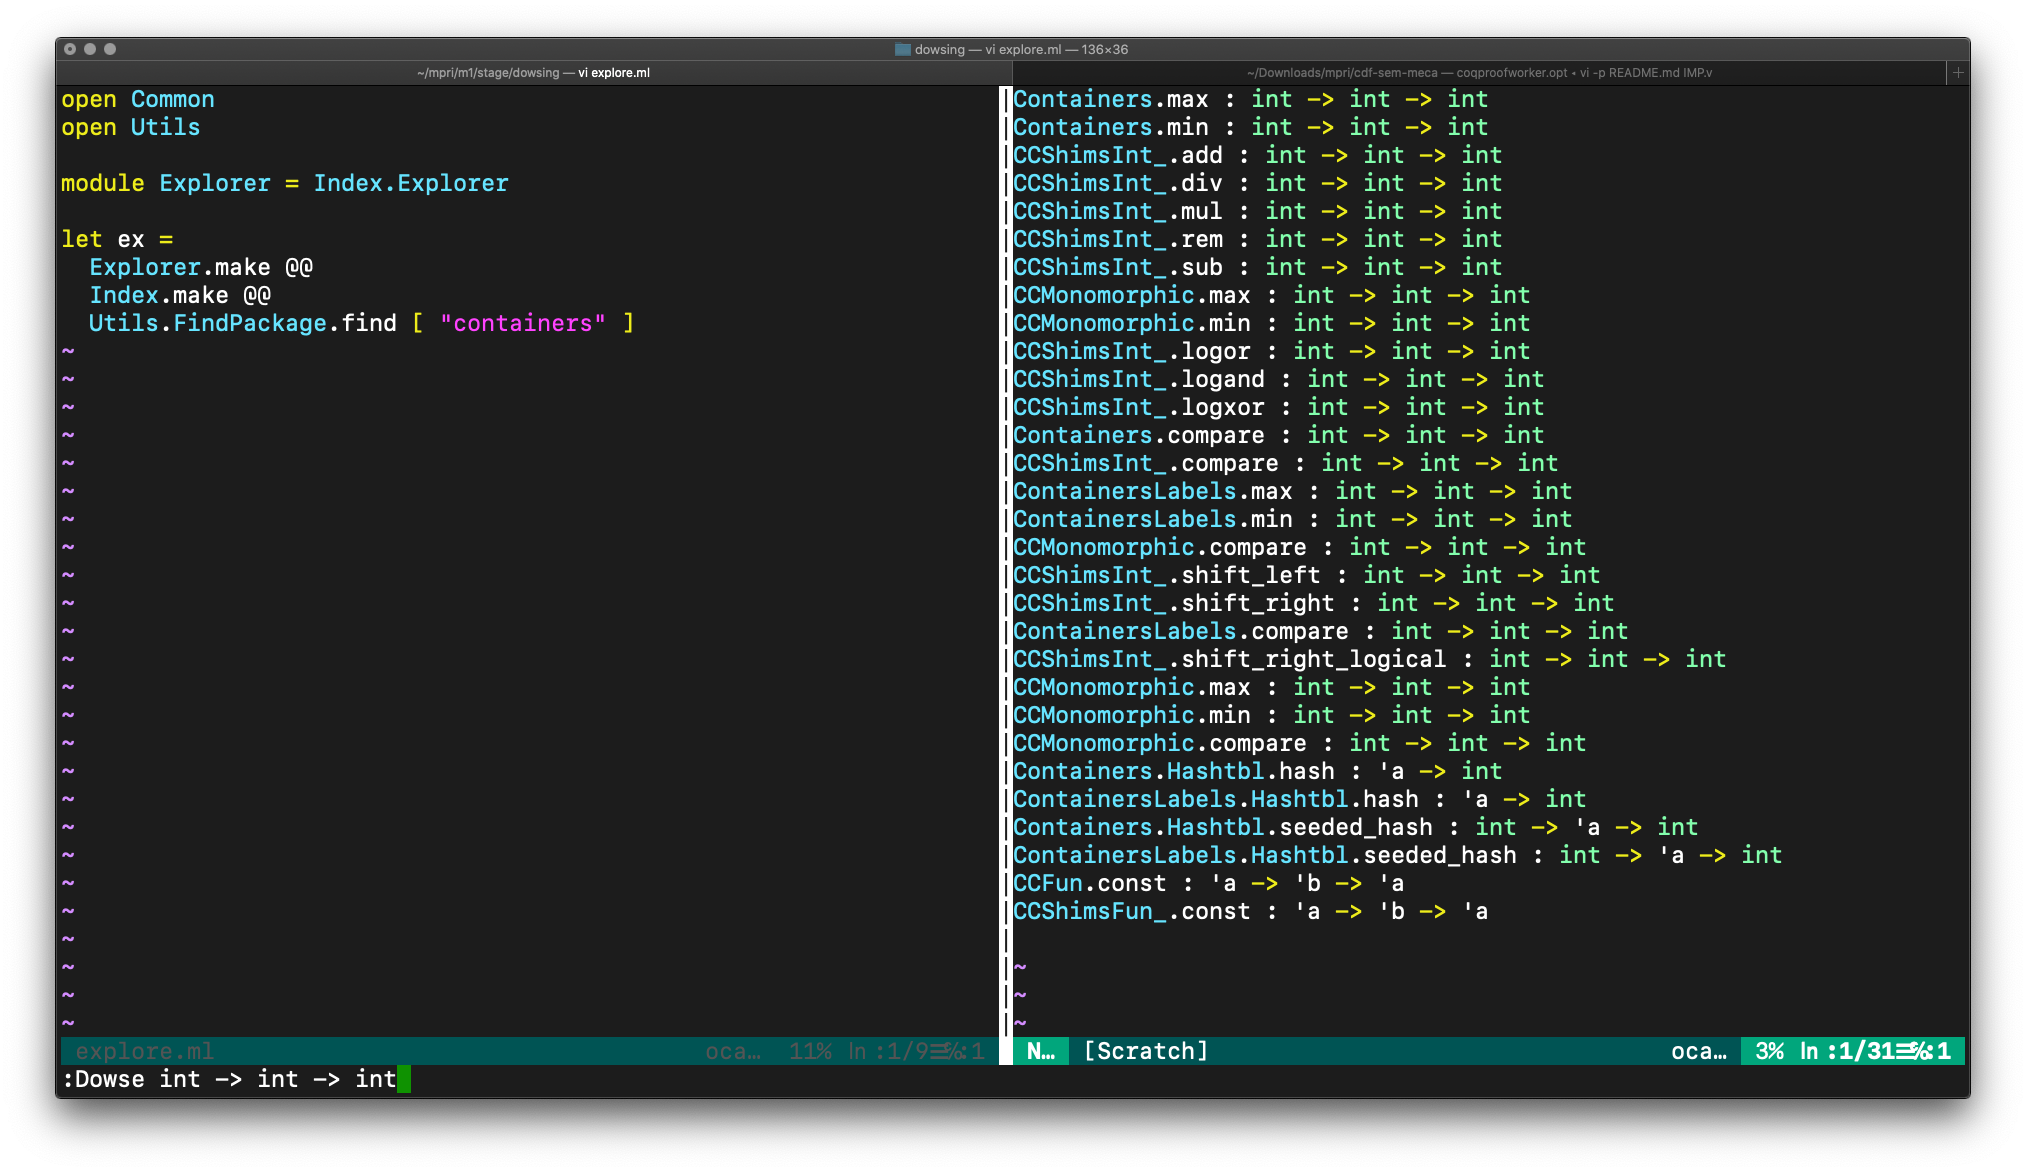
\includegraphics [scale=0.18] {images/vim_plugin}
\end {center}
\end {figure}

TODO

%============================================================
%============================================================

\chapter {Conclusion}

TODO

%============================================================
%============================================================

\chapter* {Annexe}

Cette annexe est dévolue à la démonstration des conditions nécessaires d'unifiabilité sans l'axiome ($*$-unit). Son inclusion complexifie considérablement le travail ; nous n'en sommes pas encore venus à bout.

Cet exposé est associé à un développement Coq disponible sur le dépôt \textit {github} \texttt {Drup/dowsing}. Nous y référerons parfois pour indiquer le fichier Coq correspondant à une certaine partie.

%============================================================

\section {Variables}

Dans toute la suite, on se donne un ensemble dénombrable $\V$ de symboles de variables. On signifiera par $v$ une variable dans les définitions inductives.

En Coq, cet ensemble est défini dans \texttt {Var.v}.

%============================================================

\section {Signature}

\begin {definition} [signature]
	Une signature est un ensemble $\Sigma$ de symboles muni d'une fonction d'arité $| \cdot |_\Sigma$ de $\Sigma$ dans $\mathbb N$.
\end {definition}

Dans toute la suite, on se donne une signature $( \Sigma, | \cdot |_\Sigma )$ telle que $\V \cap \Sigma = \emptyset$. On signifiera par $f$ ou $g$ un symbole de $\Sigma$ dans les définitions inductives.

Le fichier Coq correspondant est \texttt {Signature.v}.

%============================================================

\section {Types}

\begin {definition} [type]
	L'ensemble des types, noté $T$, est défini inductivement par :
	\begin {mathpar}
	    \inferrule* 
	    	{ }
	    	{\V \subseteq T}
	    \and
	    \inferrule*
	    	{ }
	    	{unit \in T}
	    \\
	    \inferrule*
	    	{\tau_1 \in T \\ \tau_2 \in T}
	    	{\tau_1 * \tau_2 \in T}
	    \and
	   	\inferrule*
	   		{\tau_1 \in T \\ \tau_2 \in T}
	   		{\tau_1 \rightarrow \tau_2 \in T}
	  	\\
	    \inferrule*
	    	{f \in \Sigma \\ \forall i \in \interval 1 {|f|_\Sigma},\ \tau_i \in T}
	    	{f (\tau_1, \dots, \tau_{|f|_\Sigma}) \in T}
	\end {mathpar}
\end {definition}

\begin {definition} [type-flèche]
	Un type-flèche (ou une flèche) est un type de la forme : $\tau_1 \rightarrow \tau_2$.
\end {definition}

\begin {definition} [racine d'un type]
	La racine d'un type, notée $[ \cdot ]$, est le symbole défini inductivement par :
	\begin {align*}
		[ v ] &= v \\
		[ unit ] &= unit \\
		[ \tau_1 * \tau_2 ] &= * \\
		[ \tau_1 \rightarrow \tau_2 \in T ] &=\ \rightarrow \\
		[ f (\tau_1, \dots, \tau_{|f|_\Sigma}) ] &= f
	\end {align*}
\end {definition}

\begin {definition} [substitution de types]
	Une substitution de types est une fonction de $\V$ dans $T$.
\end {definition}

\begin {definition} [extension d'une substitution de types]
	Soit $\sigma$ une substitution de types. \\
	L'extension de $\sigma$, notée $\hat \sigma$, est définie inductivement par :
	\begin {align*}
		\hat \sigma (v) &= \sigma (v) \\
		\hat \sigma (unit) &= unit \\
		\hat \sigma (\tau_1 * \tau_2) &= \hat \sigma (\tau_1) * \hat \sigma (\tau_2) \\
		\hat \sigma (\tau_1 \rightarrow \tau_2) &= \hat \sigma (\tau_1) \rightarrow \hat \sigma (\tau_2) \\
		\hat \sigma (f (\tau_1, \dots, \tau_{|f|_\Sigma})) &= f (\hat \sigma (\tau_1), \dots, \hat \sigma (\tau_{|f|_\Sigma}))
	\end {align*}
\end {definition}

\begin {definition} [instance de type]
	Un type $\tau_1$ est une instance d'un type $\tau_2$, noté $\tau_2 \leqslant_T \tau_1$, s'il existe une substitution de types $\sigma$  telle que $\tau_1 = \hat \sigma (\tau_2)$.
\end {definition}

%============================================================

\section {Théorie équationnelle}

\begin {definition} [axiome équationnel]
	Un axiome équationnel est un couple de types de la forme $\tau_1 \cong \tau_2$.
\end {definition}

\begin {definition} [instance d'axiome équationnel]
	Une instance d'un axiome équationnel $\tau_1 \cong \tau_2$ est un couple de types $(\tau_1', \tau_2')$ tels que $\tau_1'$ soit une instance de $\tau_1$ et $\tau_2'$ une instance de $\tau_2$.
\end {definition}

\begin {definition} [théorie équationnelle]
	Soit $\E$ un ensemble d'axiomes équationnels. \\
	La théorie équationnelle induite par $\E$, notée $\cdot \Eeq \cdot$, est la plus petite congruence sur $\Sigma$ contenant toutes les instances des axiomes équationnels de $\E$. \\
	Autrement dit, c'est la plus petite relation binaire satisfaisant les règles d'inférence :
	\begin {mathpar}
		\inferrule*
			[right = ($\Eeq$-ax)]
			{\tau_1 \cong \tau_2 \in \E}
			{\hat \sigma (\tau_1) \Eeq \hat \sigma (\tau_2)}
		\and
		\inferrule*
			[right = ($\Eeq$-refl)]
			{ }
			{\tau \Eeq \tau}
		\\
		\inferrule*
			[right = ($\Eeq$-trans)]
			{\tau_1 \Eeq \tau_2 \\ \tau_2 \Eeq \tau_3}
			{\tau_1 \Eeq \tau_3}
		\and
		\inferrule*
			[right = ($\Eeq$-sym)]
			{\tau_1 \Eeq \tau_2}
			{\tau_2 \Eeq \tau_1}
		\\
		\inferrule*
			[right = ($\Eeq$-cong-$*_1$)]
			{\tau_1 \Eeq \tau_1'}
			{\tau_1 * \tau_2 \Eeq \tau_1' * \tau_2}
		\and
		\inferrule*
			[right = ($\Eeq$-cong-$*_2$)]
			{\tau_2 \Eeq \tau_2'}
			{\tau_1 * \tau_2 \Eeq \tau_1 * \tau_2'}
		\\
		\inferrule*
			[right = ($\Eeq$-cong-$\rightarrow_1$)]
			{\tau_1 \Eeq \tau_1'}
			{\tau_1 \rightarrow \tau_2 \Eeq \tau_1' \rightarrow \tau_2}
		\and
		\inferrule*
			[right = ($\Eeq$-cong-$\rightarrow_2$)]
			{\tau_2 \Eeq \tau_2'}
			{\tau_1 \rightarrow \tau_2 \Eeq \tau_1 \rightarrow \tau_2'}
		\\
		\inferrule*
			[right = ($\Eeq$-cong-$\Sigma$)]
			{f \in \Sigma \\ i \in \interval 1 {|f|_\Sigma} \\ \tau_i \Eeq \tau_i'}
			{f (\tau_1, \dots, \tau_i, \dots, \tau_{|f|_\Sigma}) \Eeq f (\tau_1, \dots, \tau_i', \dots, \tau_{|f|_\Sigma})}
	\end {mathpar}
\end {definition}

Dans toute la suite, on s'intéressa à l'ensemble $\E$ des axiomes équationnels (où $x$, $y$ et $z$ désignent des variables) :
\begin {align*}
	x * (y * z) &\cong (x * y) * z && \text {($*$-assoc)} \\
	x * y &\cong y * x && \text {($*$-comm)} \\
	x * y \rightarrow z &\cong x \rightarrow y \rightarrow z && \text {(curry)}
\end {align*}

On considérera également la théorie équationnelle $\cdot \Eeq \cdot$ induite par $\E$.

\begin {definition} [équivalence]
	Deux types $\tau_1$ et $\tau_2$ sont équivalents {\ssi} $\tau_1 \Eeq \tau_2$.
\end {definition}

\begin {definition} [unifiabilité]
	Deux types $\tau_1$ et $\tau_2$ sont unifiables, noté $\tau_1 \ueq \tau_2$, \ssi :
	\[ \exists \sigma \in \mathscr F (\mathscr V, T),\ \hat \sigma (\tau_1) \Eeq \hat \sigma (\tau_2) \]
\end {definition}

%============================================================

\section {Premier critère (tête)}

\begin {definition} [tête d'un type]
	La tête d'un type, notée $\uparrow \cdot$, est définie inductivement par :
	\begin {align*}
		\uparrow (\tau_1 \rightarrow \tau_2) &=\ \uparrow \tau_2 \\
		\uparrow \tau &= \tau
	\end {align*}
\end {definition}

\begin {lemme} \label {=E-tete}
	Si deux types sont équivalents, leurs têtes le sont aussi.
\end {lemme}

\begin {lemme} \label {tete-subst-tete}
	$\forall \tau \in T,\ \forall \sigma \in \mathscr F (\mathscr V, T),\ \uparrow \hat \sigma (\tau) =\ \uparrow \hat \sigma (\uparrow \tau)$
\end {lemme}

\begin {lemme} \label {tete-non-fleche}
	La tête d'un type n'est pas une flèche.
\end {lemme}

\begin {lemme} \label {cons-=E}
	\begin {align*}
		\forall f_1 \in \Sigma &,\ \forall f_2 \in \Sigma, \\
		\forall (\tau^1_i)_{i \in \interval 1 {|f_1|_\Sigma}} \in T^{|f_1|_\Sigma} &,\ \forall (\tau^2_i)_{i \in \interval 1 {|f_2|_\Sigma}} \in T^{|f_2|_\Sigma}, \\
		f_1 (\tau^1_1, \dots, \tau^1_{|f_1|_\Sigma}) &= f_2 (\tau^2_1, \dots, \tau^2_{|f_2|_\Sigma}) \\
		\implies f_1 &= f_2
	\end {align*}
\end {lemme}

\begin {theoreme}
	Si deux types $\tau_1$ et $\tau_2$ sont unifiables et les racines de leurs têtes dans $\Sigma$, alors ces racines sont les mêmes :
	\begin {align*}
		\forall \tau_1 \in T &,\ \forall \tau_2 \in T, \\
		\tau_1 &\ueq \tau_2 \ \wedge \\
		[ \uparrow \tau_1 ] = f_1 \in \Sigma &\wedge [ \uparrow \tau_2 ] = f_2 \in \Sigma \\
		\implies f_1 &= f_2
	\end {align*}
\end {theoreme}

\begin {preuve}
	Par hypothèse, il existe une substitution de types $\sigma$ telle que :
	\[ \hat \sigma (\tau_1) \Eeq \hat \sigma (\tau_2) \]
	Par le lemme \ref {=E-tete}, les têtes sont équivalentes :
	\[ \uparrow \hat \sigma (\tau_1) \Eeq\ \uparrow \hat \sigma (\tau_2) \]
	Par le lemme \ref {tete-subst-tete}, on a donc :
	\[ \uparrow \hat \sigma (\uparrow \tau_1) \Eeq\ \uparrow \hat \sigma (\uparrow \tau_2) \]
	Par hypothèse, il existe $f_1$ et $f_2$ dans $\Sigma$ ainsi que $(\tau^1_i)_{i \in \interval 1 {|f_1|_\Sigma}}$ dans $T^{|f_1|_\Sigma}$ et $(\tau^2_i)_{i \in \interval 1 {|f_2|_\Sigma}}$ dans $T^{|f_2|_\Sigma}$ tels que :
	\begin {align*}
		\tau_1 &= f_1 (\tau^1_1, \dots \tau^1_{|f_1|_\Sigma}) \\
		\tau_2 &= f_2 (\tau^2_1, \dots \tau^2_{|f_2|_\Sigma})
	\end {align*}
	Par le lemme \ref {tete-non-fleche}, $f_1$ et $f_2$ sont différents de $\rightarrow$. \\
	Par definition de $\uparrow \cdot$ et $\hat \sigma$, il vient alors :
	\[ f_1 (\hat \sigma (\tau^1_1), \dots, \hat \sigma (\tau^1_{|f_1|_\Sigma})) \Eeq f_2 (\hat \sigma (\tau^2_1), \dots, \hat \sigma (\tau^2_{|f_2|_\Sigma})) \]
	Enfin, le lemme \ref {cons-=E} donne :
	\[ f_1 = f_2 \]
\end {preuve}

%============================================================

\section {Deuxième critère (queue)}

\begin {definition} [multiplicité de symbole de fonctions]
	La multiplicité d'un symbole $f$ de $\Sigma$, notée $\mu_f$, est définie inductivement par :
	\begin {align*}
		\mu_f (\tau_1 \rightarrow \tau_2) &= \mu_f' (\tau_1) + \mu_f (\tau_2) \\
		\mu_f (\tau) &= 0 \\
		\mu_f' (\tau_1 * \tau_2) &= \mu_f' (\tau_1) + \mu_f' (\tau_2) \\
		\mu_f' (f (\tau_1, \dots, \tau_n)) &= 1 \\
		\mu_f' (\tau) &= 0
	\end {align*}
\end {definition}

\begin {definition} [$\V$-multiplicité]
	La $\V$-multiplicité est définie inductivement par :
	\begin {align*}
		\mu_\V (\tau_1 \rightarrow \tau_2) &= \mu_\V' (\tau_1) + \mu_\V (\tau_2) \\
		\mu_\V (\tau) &= 0 \\
		\mu_\V' (v) &= 1 \\
		\mu_\V' (\tau_1 * \tau_2) &= \mu_\V' (\tau_1) + \mu_\V' (\tau_2) \\
		\mu_\V' (\tau) &= 0
	\end {align*}
\end {definition}

\begin {definition} [type simpe]
	Un type $\tau$ est simple si sa $\V$-multiplicité est nulle.
\end {definition}

\begin {lemme} \label {mu-=E}
	Si deux type $\tau_1$ et $\tau_2$ sont équivalents, alors, pour tout symbole $f$ de $\Sigma$, on a : $\mu_f (\tau_1) = \mu_f (\tau_2)$.
\end {lemme}

\begin {lemme} \label {mu-subst-simple}
	Si un type $\tau$ est simple, alors, pour tout symbole $f$ de $\Sigma$ et toute substitution de types $\sigma$, on a : $\mu_f (\hat \sigma (\tau)) = \mu_f (\tau)$.
\end {lemme}

\begin {lemme} \label {mu-subst}
	La multiplicité de tout symbole $f$ de $\Sigma$ dans un type est inférieure à celle de toute instance de ce type.
\end {lemme}

\begin {theoreme}
	Soit deux types $\tau_1$ et $\tau_2$. \\
	Si $\tau_1$ et $\tau_2$ sont unifiables et $\tau_1$ simple, alors la multiplicité de tout symbole de $\Sigma$ dans $\tau_1$ est supérieure à celle dans $\tau_2$.
\end {theoreme}

\begin {preuve}
	Par hypothèse, il existe une substitution $\sigma$ telle que :
	\[ \hat \sigma (\tau_1) \Eeq \hat \sigma (\tau_2) \]
	Soit $f$ un symbole de $\Sigma$. \\
	Par le lemme \ref {mu-=E}, les multiplicités sont égales :
	\[ \mu_f (\hat \sigma (\tau_1)) = \mu_f (\hat \sigma (\tau_2)) \]
	Par le lemme \ref {mu-subst-simple}, la simplicité de $\tau_1$ apporte :
	\[ \mu_f (\hat \sigma (\tau_1)) = \mu_f (\tau_1) \]
	Par le lemme \ref {mu-subst}, on a par ailleurs :
	\[ \mu_f (\hat \sigma (\tau_2)) \geqslant \mu_f (\tau_2) \]
	Il vient donc le résultat attendu :
	\[ \mu_f (\tau_1) \geqslant \mu_f (\tau_2) \]
\end {preuve}

%============================================================
%============================================================

\printbibliography

\end {document}

























